\chapter{Vision}
	Im Rahmen der Semesterarbeit ``A Practical JavaScript-Only Video-Over-IP Communication Plattform"' wird eine
	Video-Over-IP-Applikation entwickelt, die vollständig im Browser läuft.
	
	Die Applikation läuft in modernen Browser ohne Plugins oder die Installation lokaler Software.
			
	\begin{figure}[H]
		\centering
		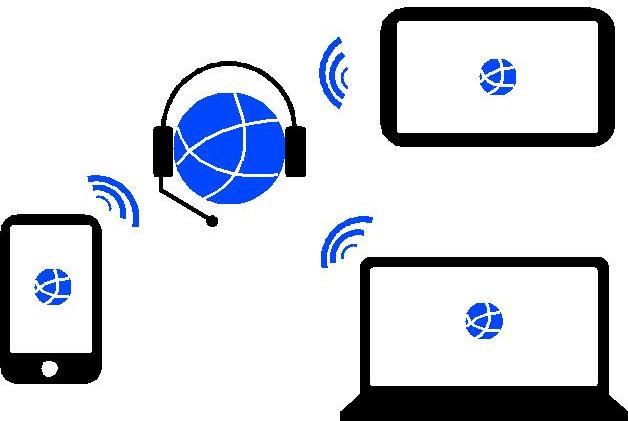
\includegraphics[width=0.5\textwidth]{img/plattformUnabhaengigkeit.jpg}
		\label{plattformUnabhaengigkeit}
	\end{figure}
	
	Durch den offenen Standard ``WebRTC"' ist die Applikation auf jedem modernen Gerät benutzbar, das den Standard umsetzt und genug Leistung für Audio- und Videokommunikation bereitstellt.
	
	Durch die einfache Benutzung ist die Applikation auch für technisch nicht
	versierte Benutzer zugänglich.
	
	Das integrierte Kontaktmanagement kann mit verschiedenen Importformaten umgehen und einfach um weitere Quellen erweitert werden. Dazu gibt es eine Adressbuchschnittstelle.
	
	Die Applikation kann um beliebige Signallingchannel erweitert werden. Somit ist
	es unter anderem möglich, die Applikation um Signalling über SIP oder XMPP zu
	erweitern. Dazu gibt es eine Channelschnittstelle.
	
	
	\section{Ziele}
		\begin{itemize}
			\item Audio- und Videokommunikation zwischen zwei Teilnehmern.
			\item Signalling\footnote{Benachrichtigen eines andern Peers über eine Verbindungsanfrage und Austausch von Verbindungsparametern} über beliebige Channels, Referenzimplementation eines Channels mit XHR\footnote{XML HTTP Request, Asynchrones nachladen von HTTP Seiten}.
			\item Adressbuchimport von beliebigen Quellen, Referenzimplementationen für JSON
				\footnote{Javascript Object Notation, strukturiertes mensch- und maschinenlesbares Datenaustauschformat, 
					IETF, JSON (Stand Juli 2006)
					\hyperlink{http://tools.ietf.org/html/rfc4627}{http://tools.ietf.org/html/rfc4627}, [Abruf am 21.11.13]
				} und VCARD
				\footnote{Elektronische Visitenkarte, IETF, vCard Format Spezifikation (Stand August 2011) 
					\hyperlink{http://tools.ietf.org/html/rfc6350}{http://tools.ietf.org/html/rfc6350}, [Abruf am 21.11.13]
				} Import sowie eines Online Adressbuches über eine JSON Schnittstelle.
			\item Speichern von Adressbüchern und Benutzerinformationen im Browser (Local Storage).
			\item Verschlüsselte Kommunikation zwischen den Clients. Die Kommunikation der Signalling Channel Referenzimplementation muss nicht zwingend verschlüsselt werden, da diese automatisch verschlüsselt wird sobald die Verbindung mit TLS geschützt wird.
		\end{itemize}
		
	\section{Abgrenzung}
		\begin{itemize}
			\item Kommunikation mit mehreren Teilnehmern ist nicht Teil der Arbeit, es soll jedoch sichergestellt werden, das dies später umgesetzt werden könnte.
			\item Für Adressbuchimport und Signalling-Channel soll nur die API und eine
			Referenzimplementation umgesetzt werden und keine Implementationen für diverse Formate.
		\end{itemize}
		
	\section{Optionale Erweiterungen}
		Optional könnte die Applikation um einige praktische Funktionen erweitert werden:		
		\begin{itemize}
			\item Chat
			\item Austausch von Dateien
			\item Screensharing soweit die Browser solche Funktionalität überhaupt schon unterstützen
		\end{itemize}